\section{Einführung und Grundlagen}
	
	Bevor der eigentliche Versuch besprochen wird, sollen noch einige Grundlagen erörtert werden.
\subsection{Reflexion und Transmission an Grenzflächen} \label{sec:fresnel}
	Trifft elektromagnetische Strahlung auf eine ladungs- und stromfreie Grenzfläche, so erfüllen die elektrischen und magnetischen Felder, die die Welle beschreiben, bestimmte Stetigkeitsbedingungen und es treten Reflexions- und Transmissionseffekte auf. Im Allgemeinen muss man dabei eine Fallunterscheidung vornehmen, die die parallel und senkrecht zur Oberfläche polarisieren Anteile der einfallenden Welle voneinander trennt. Im vorliegenden Experiment wird allerdings ein Lichtstrahl (mit Amplitude $E_0$) betrachtet, der senkrecht von Luft (Brechungsindex $n_{Luft} = \unit[1,000292]{} \simeq 1$) in ein optisch dichteres Medium mit Brechungsindex $n$ propagiert. Dabei verhalten sich parallel und senkrecht polarisierte Komponenten - bis auf Phasenfaktoren, die bei einer Intensitätsmessung ohnehin verloren gehen - äquivalent, weshalb die Fallunterscheidung entfällt. Die Amplitudenverhältnisse der dabei auftretenden partiellen Grenzflächeneffekte werden durch die \textit{Reflexions- und Transmissionkoeffizienten} beschrieben:
	\begin{align}
		&r_s \equiv r := \frac{E_r}{E_0} = \frac{n_{Luft} - n}{n_{Luft} + n} \simeq \frac{1 - n}{1 + n}, \label{eq:r_s}\\
		&t_s \equiv t := \frac{E_t}{E_0} = \frac{2n_{Luft}}{n_{Luft} + n} \simeq \frac{2}{1 + n}. \label{eq:t_s} 
	\end{align}
	Gleichungen (\ref{eq:r_s}) und (\ref{eq:t_s}) stellen somit den Spezialfall der \textit{Fresnelschen Formeln} für senkrechten Einfall dar. Analog ergibt sich für den Übergang vom optisch dichteren Medium zu Luft:
	\begin{align}
			&r_s^\prime \equiv r^\prime \simeq \frac{n - 1}{1 + n} = -r_s,\\
			&t_s^\prime \equiv t^\prime \simeq \frac{2n}{1 + n} = n \cdot t_s. 
	\end{align}
	Da mit den vorliegenden Detektoren nur Intensitäten $I = \vec{\abs{E}}^2$ gemessen werden und somit Phaseninformationen verloren gehen, definiert man den sogenannten \textit{Reflexions- und Transmissionsgrad} als Verhältnis der reflektierten/transmittierten Leistung des elektrischen Feldes zu der des einfallendes Feldes. Im vorliegenden Spe\-zial\-fall senkrechtem Einfalls (s.E.) ergeben sich diese zu:
	\begin{align}
		&R := \frac{P_r}{P_e} = \abs{\frac{E_r}{E_0}}^2 = \frac{I_r}{I_0} = r^2 \overset{(\ref{eq:r_s})}{=} \frac{(n-1)^2}{(n+1)^2} = R^\prime, \label{eq:R}\\
		&T := \frac{P_t}{P_e} \overset{s.E.}{=} \abs{\frac{E_t}{E_0}}^2 = \frac{I_t}{I_0} = t^2 \overset{(\ref{eq:t_s})}{=} \frac{4}{(n+1)^2} = \frac{1}{n^2}T^\prime, \label{eq:T}
	\end{align}
	Diese vier Größen werden im Experiment durch Vergleich der Intensität des Probestrahls mit einem Referenzstrahl, welcher kein Medium durchläuft, aber sonst den gleichen Weg passiert, ermittelt.\\
	Im ersten Teil des Versuches wird der Brechungsindex $n$ einer Glasprobe ermittelt werden. Dafür wird nun ein funktionaler Zusammenhang $n = n(R, R', T, T')$ gesucht. Dafür wird ein auf das Glas senkrecht einfallender Strahl mit Intensität $I_0$ betrachtet. Trifft dieser auf die Grenzfläche, wird ein Teil reflektiert ($I_r \overset{(\ref{eq:R})}{=} R I_0$) und ein Teil transmittiert ($I_t \overset{(\ref{eq:T})}{=} T I_0$). Anschließend tritt dies erneut an der Grenzfläche Glas-Luft auf, d.h. ein Teil des vorher transmittierten Strahles wird reflektiert ($I = T R^\prime I_0$) oder es verlässt das Medium ($I = T T^\prime I_0$). Dieser Vorgang wiederholt sich unendlich oft und wird in Abbildung \ref{fig:brechungsindex} skizziert.
	\begin{figure}[ht]
		\centering
		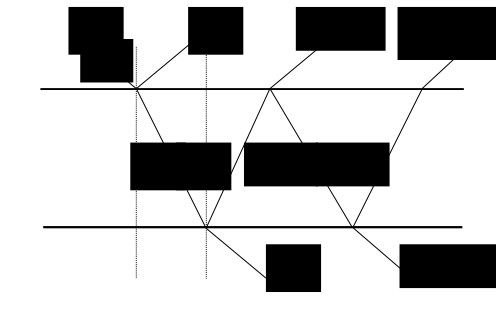
\includegraphics[width=\linewidth]{pic/Brechungsindex.pdf}
		\caption{Intensitätsverhältnisse einer an einer Grenzfläche unendlich oft transmittierten und reflektierten elektromagnetischen Welle.}
		\label{fig:brechungsindex}	
	\end{figure}
	Bei einem senkrecht einfallenden Strahl ergibt sich somit die Intensität des Strahles, der das Medium verlässt als Überlagerung aller Strahlen mit geraden Potenzen von $R = R^\prime$. Analog ist der reflektierte Strahl die Superposition aller Strahlen mit den ungeraden Potenzen.
	\begin{align}
		&I_{t,ges} = \sum_{k = 0}^{\infty} T\cdot T^\prime \cdot (R^{\prime 2})^k \cdot I_0 =: T_{ges}\cdot I_0\\
		&I_{r,ges} = \left(R + \sum_{k = 0}^{\infty} T\cdot T^\prime \cdot (R^\prime)^{2k+1}\right) \cdot I_0 =: R_{ges}\cdot I_0
	\end{align}
	Unter Verwendung der Gleichungen (\ref{eq:R}) und (\ref{eq:T}) und der geometrischen Reihe ergibt sich das gemessene gesamte Reflexions- und Transmissionsvermögen zu:
	\begin{align}
			&T_{ges}(n) = T\cdot T^\prime \cdot \frac{1}{1 - R^2} = \frac{2n}{n^2 + 1},\\
			&R_{ges}(n) = R\cdot \left(1 + T\cdot T^\prime \cdot \frac{1}{1 - R^2}\right) = R (1 + T_{ges}) = \frac{(n-1)^2}{n^2+1},\\
			&T_{ges} + R_{ges} = 1.
	\end{align}
	Daraus erhält man durch Lösen der sich ergebenden quadratischen Gleichung den Brechungsindex:
	\begin{align}
		&n(T_{ges}) = \frac{1}{T_{ges}}\left(1 + \sqrt{1 - T_{ges}^2}\right), \label{eq:n_T}\\
		&n(R_{ges}) = \frac{1}{1 - R_{ges}}\left(1 + \sqrt{1 - (1 - R_{ges})^2}\right) \label{eq:n_R}
	\end{align}
\subsection{Aufbau der Versuchsanordnungen}
    Während des Praktikums werden verschiedene Versuchsaufbauten verwendet, um jeweils den Transmissions- und Reflexionsgrade verschiedener Materialien sowie die Anregungswellenlänge einer organischen, fluoreszierenden Probe zu ermitteln.
    \subsubsection{Shimadzu 3100}
        Für die Aufnahme der Reflexions- und Transmissionsgrade werden zwei verschiedene Aufbauten eines Gerätes, dem Shimadzu 3100, verwendet. Dieses Gerät erzeugt mithilfe einer Halogen- und einer Deuteriumlampe Licht verschiedener Wellenlängen, wobei die einzelnen Wellenlängen mithilfe optischer Gitter anstelle von Prismen realisiert werden. Im Gegensatz zur Verwendung eines Prismas hängt die Beugung über das Gitter nicht direkt von der Wellenlänge ab und es entstehen auch weniger Unsicherheiten aufgrund der Unabhängigkeit von der Brechzahl. In Abbildung \ref{aufb:transmiss} ist der Transmissionsaufbau zu sehen. 
        \textbf{Anordnung zur Messung der Transmission}
            \begin{figure}
                \includegraphics[scale=0.15]{pic/transmiss_aufbau.png}
                \caption{Aufbau zur Transmissionsmessung}
                \label{aufb:transmiss}
            \end{figure}
    \subsubsection{Fluoromax}